\documentclass[12pt, a4paper]{article}
\usepackage[francais]{babel}
\usepackage{caption}
\usepackage{graphicx}
\usepackage[T1]{fontenc}
\usepackage{listings}
\usepackage{geometry}
\usepackage{amsmath}
\usepackage{listings}
\usepackage[colorlinks=true,linkcolor=black,anchorcolor=black,citecolor=black,filecolor=black,menucolor=black,runcolor=black,urlcolor=black]{hyperref}

% \usepackage{mathpazo} --> Police à utiliser lors de rapports plus sérieux

\usepackage{fancyhdr}
\pagestyle{fancy}
\lhead{}
\rhead{}
\chead{}
\rfoot{\thepage}
\lfoot{Martin Baumgaertner}
\cfoot{}

\renewcommand{\headrulewidth}{0.4pt}
\renewcommand{\footrulewidth}{0.4pt}

\begin{document}
\begin{titlepage}
	\newcommand{\HRule}{\rule{\linewidth}{0.5mm}} 
	\center 
	\textsc{\LARGE iut de colmar}\\[6.5cm] 
	\textsc{\Large R405 Automatisation des tâches}\\[0.5cm] 
	\textsc{\large Année 2022-23}\\[0.5cm]
	\HRule\\[0.75cm]
	{\huge\bfseries TP 2 : Bash}\\[0.4cm]
	\HRule\\[1.5cm]
	\textsc{\large martin baumgaertner}\\[6.5cm] 

	\vfill\vfill\vfill
	{\large\today} 
	\vfill
\end{titlepage}
\newpage
\tableofcontents
\newpage
\section{Exercice 1}
Voici donc le script qui vérifie toutes les conditions une à une. 
\begin{figure}[h]
    \centering
    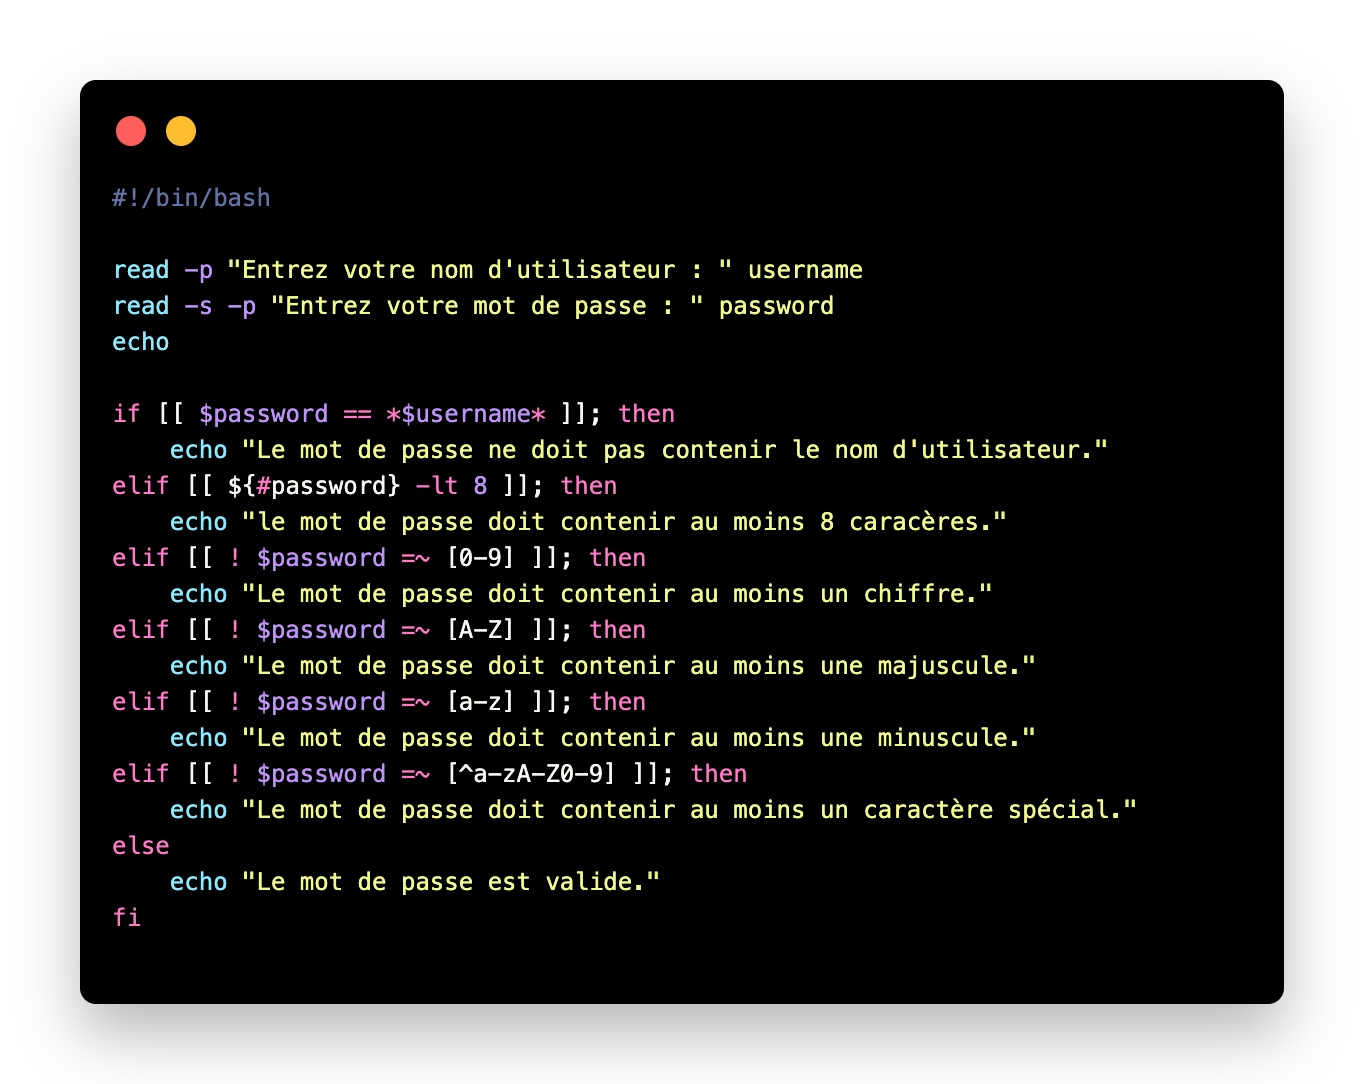
\includegraphics[width=1\textwidth]{img/exo1.png}
    \caption{Exercice 1}
    \label{fig:script2}
\end{figure}

\newpage
\section{Exercice 2}
\begin{figure}[h]
    \centering
    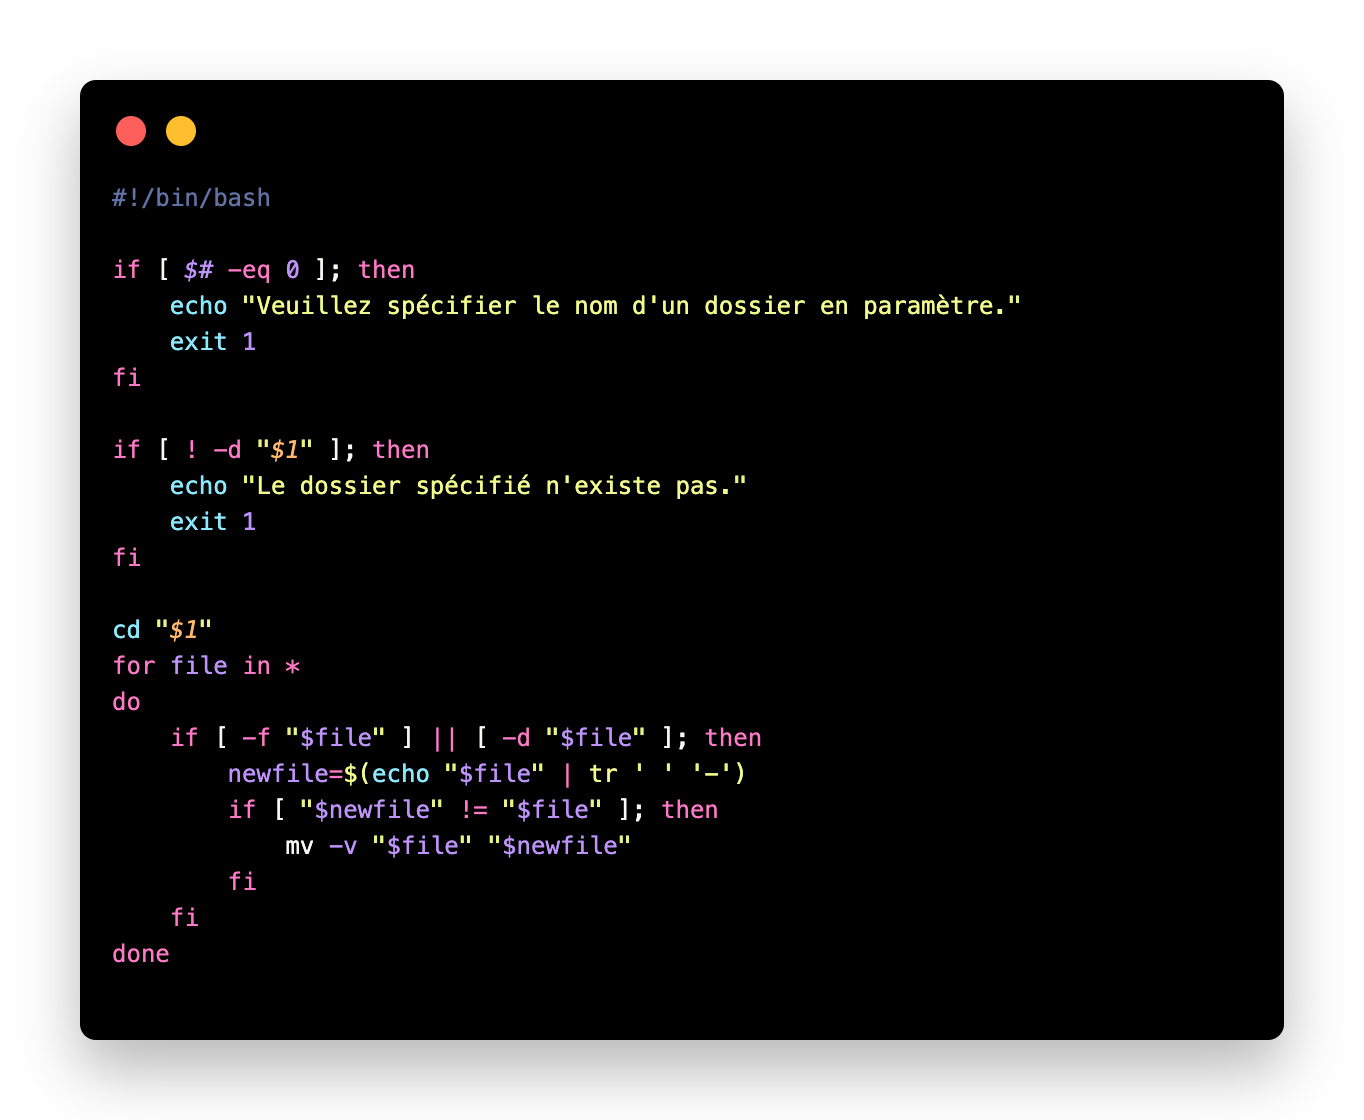
\includegraphics[width=1\textwidth]{img/exo2.png}
    \caption{Exercice 2}
    \label{fig:script3}
\end{figure}

On vient vérifier la condition qui vérifie si le nombre de paramètres 
passés en entrée est inférieur à 3. Si c'est le cas, le script affiche 
un message d'erreur demandant à l'utilisateur de spécifier le nom d'un 
dossier, le caractère à remplacer, et le caractère de remplacement en 
paramètres, puis le script se termine avec un code d'erreur 1.

\newpage
\section{Exercice 3}
\begin{figure}[h]
    \centering
    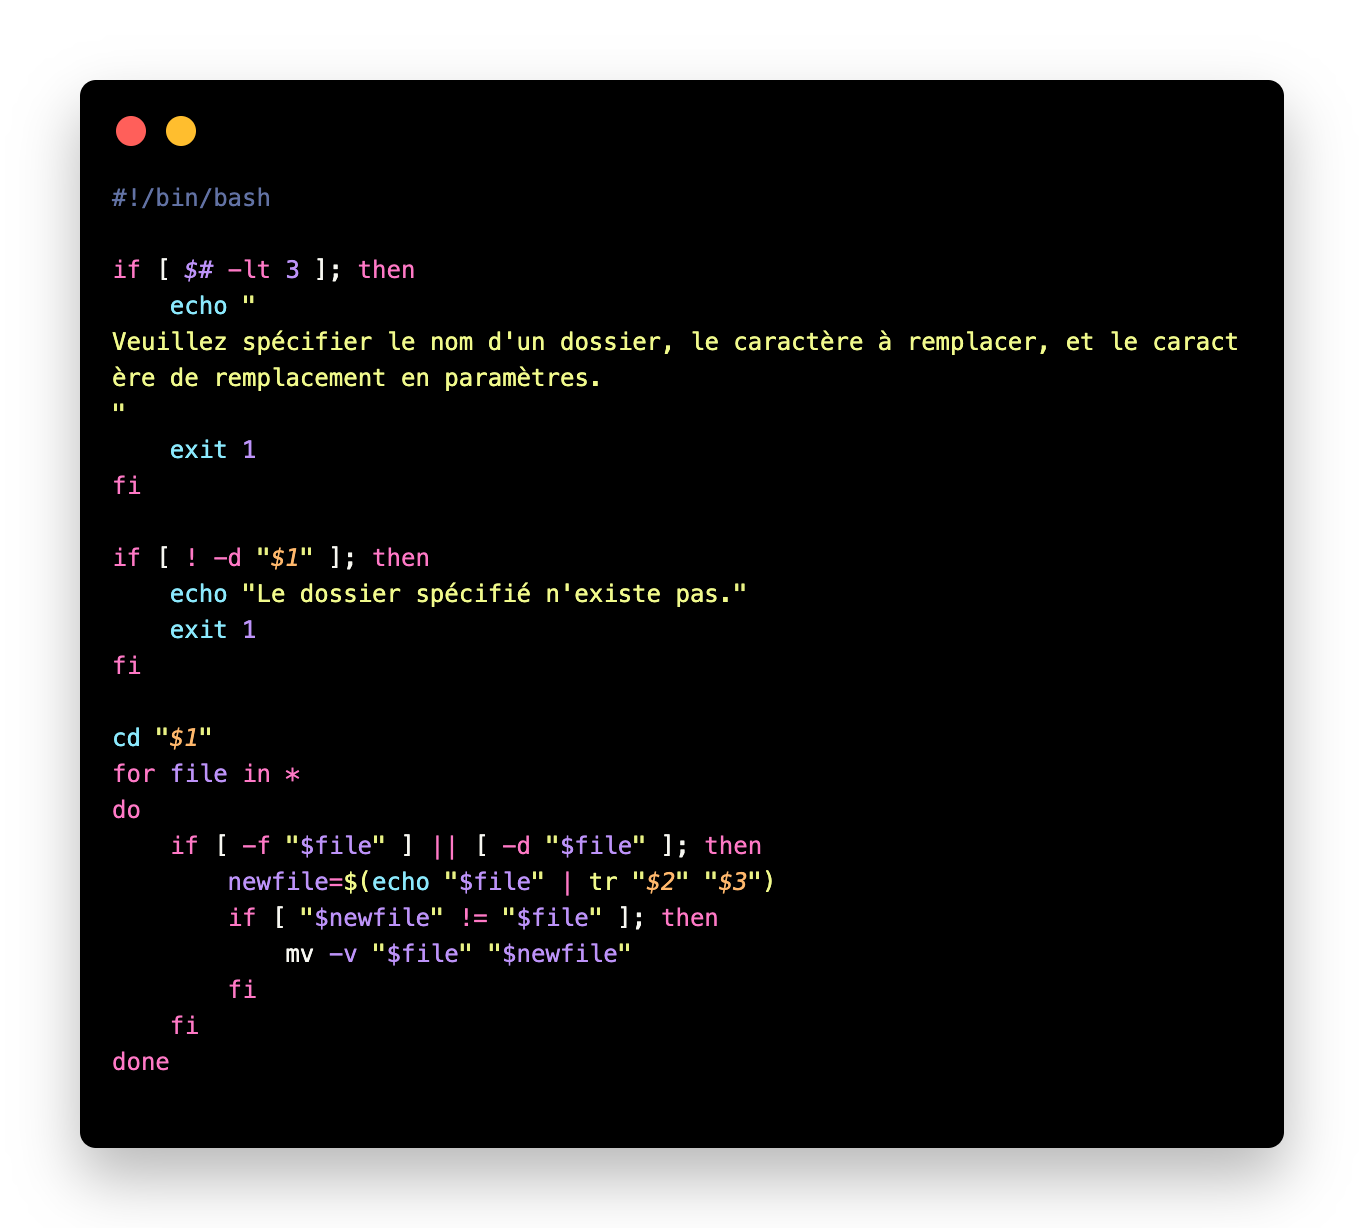
\includegraphics[width=1\textwidth]{img/exo3.png}
    \caption{Exercice 3}
    \label{fig:scrip3}
\end{figure}
Le code présent dans la condition else vérifie si l'option -r 
n'est pas spécifiée. Dans ce cas, le script change le répertoire de 
travail courant pour le répertoire spécifié dans le premier paramètre. 
Ensuite, le script itère sur chaque fichier et dossier dans le répertoire 
courant, en vérifiant s'il s'agit d'un fichier ou d'un dossier. Le script 
remplace les caractères spécifiés dans le deuxième paramètre par les 
caractères de remplacement spécifiés dans le troisième paramètre pour 
chaque fichier ou dossier, et les renomme avec le nouveau nom s'il est 
différent de l'ancien nom. En fin de compte, si l'option -r n'est pas 
spécifiée, le script ne parcourt que le répertoire courant et renomme 
les fichiers et dossiers dans ce répertoire en fonction des caractères 
spécifiés.



\end{document}